%Preamble

\RequirePackage[l2tabu, orthodox]{nag}
\documentclass{article}
\usepackage[utf8]{inputenc}
\usepackage[usenames, dvipsnames]{xcolor}
\usepackage[english]{babel}
\usepackage[documents]{ragged2e}
% 9 LaTeX packages everyone should use
\usepackage{amsmath}
\usepackage[a4paper]{geometry}
\usepackage[rightcaption]{sidecap}
\usepackage[skip=true,justification=justified,singlelinecheck=false,font=small,format=plain,labelfont=bf,up,textfont=normal,up]{caption}
\usepackage{graphicx}
\graphicspath{ {Figures/} }
\usepackage{microtype}
\usepackage{siunitx}
\usepackage{booktabs}
\usepackage[
backend=biber,
style=authoryear,
sorting=ynt
]{biblatex}
\addbibresource{refs.bib}
\usepackage{gensymb}
\usepackage{csquotes}
\usepackage{hyperref}
\hypersetup{
    colorlinks=true,
    linkcolor=blue,
    filecolor=magenta,      
    urlcolor=cyan,
}
\urlstyle{same}
\usepackage{cleveref}

\title{Degree days explained}
\author{Michael Hunt}
\date{August 2014}

\begin{document}

\maketitle


\section{Introduction: What are Degree Days?}

They are a property of a location and are a measure of the severity and duration of cold weather at that location. The colder the weather in a given month and the longer the cold snap lasts, the greater the degree days in that month. The degree days for a month are the summation over that month of the time and extent to which the temperature outside falls below some reference or "base" temperature.

\begin{figure}[ht]
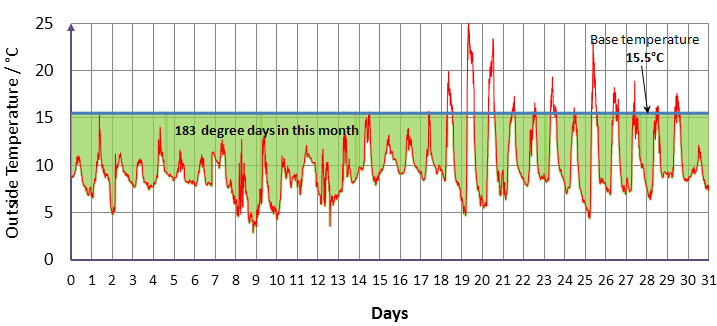
\includegraphics[width=0.9\textwidth]{one_month_BT15pt5}
\caption{The outside temperature recorded in Camborne over a one month period in early 2009.The green shaded area is the degree days for the period, for a base temperature of 15.5\degree C. In this period of 31 days there were 182.6 degree days for this base temperature, meaning that the average outside temperature was 182.6 / 31 = 5.9\degree C colder than the base temperature. Notice that periods where the outside temperature exceeds the base temperature do not count towards degree days}
\label{fig:DDdata}
\end{figure}


The rate of heat loss from a building is directly proportional to the temperature difference between the inside and the outside - the bigger this temperature difference is, the more rapidly the heat will flow, and the harder a heating system will have to work (ie the more rapidly it will have to burn fuel)  to replace this heat. The energy consumed by a heating system for space heating will be dictated not only by this temperature difference but also by its duration - if it is cold for longer, then more fuel needs to be burned. A moderately cold period that went on for a long time might in the end demand as much heating fuel as a very cold snap that didn't last so long, and so on. The idea of degree days captures this: a temperature difference of one degree for one day is one degree day. A temperature difference of ten degrees for one day or five degrees for two days, or one degree for ten days all give ten degree days - all would demand the same amount of fuel for space heating. Thus energy consumed for space heating in a given period is proportional to the number of degree days in that period.

In fact the temperature difference used in calculating the degree days over a period is not strictly that between the actual inside temperature and the outside temperature, but the difference between a \textbf{base temperature} and the actual outside temperature. This is shown as the blue line in Figure \ref{fig:DDdata}.

The base temperature is the outside temperature below which it is necessary to heat a house in order to maintain a comfortable temperature inside. The reference temperature that is usually used is 15.5 \degree C. This is lower than the temperature normally sought inside a house, because the house is anyway self-heated by the people in it (at about 100W per person), the lighting and appliances and so on. These self-heating sources are sufficient to raise the temperature of the house to the 18-19 \degree C we normally now require to feel comfortable, in this country at least, even if the outside temperature is a few degrees colder than that. If it gets any colder then these sources are no longer sufficient and it becomes necessary to turn on the heating. 15.5 \degree C is conventionally taken as the base temperature for dwellings, but, of course, the actual degree of self heating varies from building to building, and so in some houses, particularly well insulated draft-free houses, it can be far colder than that outside before any heating is needed. The base temperature for these houses would be lower than 15.5 \degree C. Hospitals, in contrast are required to be warmer than dwellings, so their base temperature is higher - 18.5 \degree C. This means that the number of degree days for a hospital will be higher in any period than for the houses in the estate next door, as shown in Figure \ref{fig:high_BT}

\begin{figure}[ht]
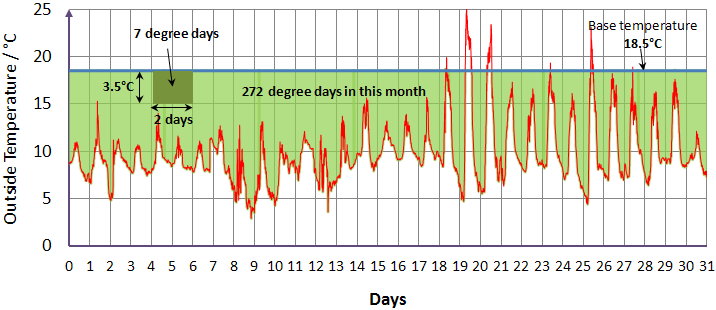
\includegraphics[width=0.9\textwidth]{one_month_BT18pt5}
\caption{The same temperature data as shown in Figure \ref{fig:DDdata}, but now with a base temperature of 18.5 \degree, as might be appropriate for a hospital. The number of degree days is now 272, whereas it was 183 for a base temperature of 15.5 \degree C.}
\label{fig:high_BT}
\end{figure}

The base temperature-outside temperature difference fluctuates on a daily and seasonal basis, and the number of degree days in a period at a location is usually found from an analysis of hourly temperature measurements taken at Met Office weather stations. Degree day data are published for 18 regions within the UK. I usually get them from the \href{http://www.eci.ox.ac.uk/research/energy/degreedays.php}{ECI}. Colder regions have higher degree day numbers than warmer regions, and colder years have higher degree day values than warmer years, as shown in Figures \ref{fig:DD_by_month} and \ref{fig:DD_by_place}.

\begin{figure}[ht]
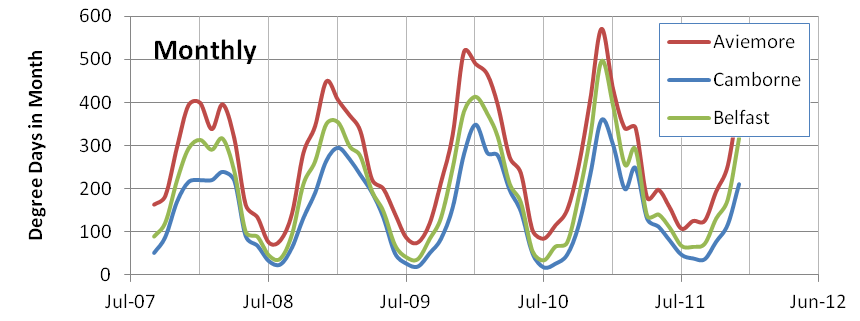
\includegraphics[width=0.9\textwidth]{DD_by_month_to_12_2011}
\caption{Monthly DD figures for Camborne compared with those for Belfast (NI) and Aviemore (Scotland) for a base temperature of 15.5\degree C. Note that winter months have more degree days than summer months and that within the UK, more northerly locations have higher DD figures than southerly locations such as Camborne.}
\label{fig:DD_by_month}
\end{figure}

\begin{figure}[ht]
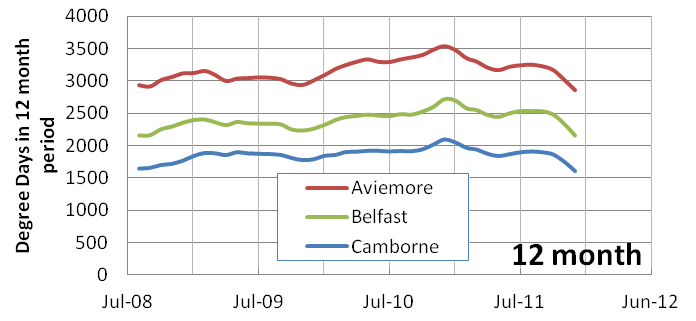
\includegraphics[width=0.9\textwidth]{DD_by_Place_to_12_2011}
\caption{Annual DD figures for Camborne compared with those for Belfast (NI) and Aviemore (Scotland) for a base temperature of 15.5\degree C. Note that  within the UK, more northerly locations have higher DD figures than southerly locations such as Camborne. This would have a direct impact on space heating energy usage - the same building placed in Aviemore, used with the same heating regime, would use approximately 50-60\% more energy for space heating than if placed in Camborne. There is also fluctuation from year to year as one year has more or less severe weather than another.}
\label{fig:DD_by_place}
\end{figure}


The annual energy  bill for space heating of a building is directly proportional to the degree days of the location where the building is located. Thus the same building, built in Aviemore (the ski resort in the Cairngorm Mountains, Scotland. Think cold.) and heated in exactly the same way as an identikit copy built in Camborne (where it rains a lot, but snows rarely and where palm trees have been spotted), would require about 50\% more energy than the Camborne copy, given that Aviemore has about 3000 degree days per year while Camborne has about 2000. It is generally warmer in Camborne than it is in Aviemore. Wetter, maybe, but definitely warmer.

\section{How are Degree days used?}

In one straightforward way, they are used to calculate the energy requirement for space heating of a building that arises from conduction losses through the skin of the building, which comprises the walls, floor, roof and all openings such as doors and windows, and through exchange of cold air outside with warm air inside, either by ventilation or by infiltration.

If we know the heat loss coefficient of the building, call this $q$, which is the rate of heat loss from a building per kelvin temperature difference between the inside and the outside, then the actual rate of heat loss at any instant will be $q\Delta T$ where $\Delta T$ is the actual temperature difference, and the total heat load on the building in one year is

\begin{equation}
E\ =\ \int{q \Delta T(t) dt}\ =\ q\int{\Delta T(t) dt}
\label{eq:full_integral}
\end{equation}
 
which can more straightforwardly be written as

\begin{equation}
E\ =\ q\times DD\times\frac{24}{1000}
\label{eq:DD_version}
\end{equation} 
ie the integral in \ref{eq:full_integral} is the degree days ($$DD$$) for the location over one year. The factor 24 / 1000 is included to ensure that the unit for $$E$$ is kWh. The factor 24 converts the days of $$DD$$ into hours, and the factor 1000 converts the watts of $q$ into kW.
Note that in equation \ref{eq:DD_version}, the first term $q$ is a property of the building, while the second term DD is a property of the location, so that \ref{eq:DD_version} captures the fact that the heat load of a building will depend on how the building is built and where it is built.

\section{Exercises}
\subsection{Example 1}


The 20 year average DD value for Cornwall is about 1700. What is the predicted annual heating load for a building with heat loss coefficient of \SI{130}{\watt\per\kelvin}?\\
 
\underline{Solution:} $$E\ =\ q\times DD\times\frac{24}{1000}\ =\ 130\times 1700\times \frac{24}{1000}\ =\ 5304\ \text{kWh}$$


\section{Additional Sources}

Useful references for the subject of degree days are the Carbon Trust \cite{CarbonTrust2012} and the ECI \cite{ECIOxfordUniversity2014} which is the Environmental Change Institute at Oxford University.

 

 \printbibliography

 

\end{document}
